%%
%% 9May2008.tex
%% 
%% Made by Alex Nelson
%% Login   <alex@tomato>
%% 
%% Started on  Sun Dec 21 20:20:11 2008 Alex Nelson
%% Last update Sun Dec 21 20:20:11 2008 Alex Nelson
%%
\begin{defn}\index{Convolution}
The \textbf{convolution} of two functions is a function
defined by
\begin{equation}
(f*g)(x) = \int_{\mathbb{R}}f(x-y)g(y)dy
\end{equation}
provided that both integrals converge.
\end{defn}

\begin{ex}
Let $f(x)=x$, $g(x)=x^2$, $h(x)=\exp(-x^2)$, then
\begin{equation}
(f*g)(x) = \int^{\infty}_{-\infty}(x-y)y^2dy
\end{equation}
does not exist for arbitrary $x$. Thus the convolution is
not well defined. However,
\begin{equation}
(f*h)(x) = \int^{\infty}_{-\infty}(x-y)e^{-y^2}dy =
  \sqrt{\pi}x
\end{equation}
for all $x\in\mathbb{R}$.
\end{ex}
\begin{proof}{(Proof of outrageous claim)}
Compute
\begin{equation}
\int^{\infty}_{-\infty}e^{-y^2}dy = \sqrt{\pi}.
\end{equation}
We can take it on faith (which I'll do out of laziness), or
we can bust open a can of complex analytical whoop ass on
the problem and use residues. We have
\begin{equation}
(f*h)(x)=x\int_{\mathbb{R}}e^{-y^{2}}dy - \int_{\mathbb{R}}ye^{-y^2}dy
\end{equation}
we see that $y\exp(-y^2)$ is odd, so its integral from
$-\infty$ to $+\infty$ vanishes. We are left with
\begin{equation}
(f*h)(x)=x\int_{\mathbb{R}}e^{-y^2}dy
\end{equation}
and this is necessarily
\begin{equation}
(f*h)(x) = x\sqrt{\pi}
\end{equation}
which concludes our proof.
\end{proof}

Note
\begin{equation}
|(f*g)(x)|\leq\int|f(x-y)g(y)|dy
\end{equation}
so if the integral converges absolutely, then the
convolution exists. \marginpar{convolution gauranteed when...}Some cases when the convolution is guarenteed:
\begin{enumerate}
\item $f\in L^{1}(\mathbb{R})$, $|g(x)|\leq M$ for all
  $x\in\mathbb{R}$, the integral converges absolutely
\item $g\in L^{1}(\mathbb{R})$, $|f(x)|\leq M$ for all
  $x\in\mathbb{R}$, then the convlution exists
\begin{equation}
\int|f(x-y)g(y)|dy\leq M\int|f(x-y)|dy<+\infty
\end{equation}
\item $f,g\in L^{2}(\mathbb{R})$, we have
\begin{equation}
\int|f(x-y)g(y)|dy\leq\left(\int|f(x-y)|^2dy\right)^{1/2}\left(\int|g(y)|^2dy\right)^{1/2}<+\infty
\end{equation}
where we justify making it less than infinity by the
properties of $L^2$.
\end{enumerate}
There are many more times whene convolution is gauranteed.

But \textbf{WTF does the convolution mean anyways?}

Recall that the average of a function on $[a,b]$ is
\begin{equation}
avg(f) = \frac{1}{b-a}\int^{b}_{a}f(x)dx
\end{equation}
We can generalize this to be a weighted average on $[a,b]$:
\begin{equation}
wt(f) = \frac{\int^{b}_{a}f(x)\omega(x)dx}{\int^{b}_{a}\omega(x)dx}
\end{equation}
For our typical average, we usually just set
$\omega(x)=1$. So for
\begin{equation}
(f*g)(x)
  = \begin{pmatrix}$weighted$\ $average$\ $of$\ g\ $around$\\
$the$\ $point$\ x $ with$\ $the$\ $weight$\\ 
$determined$\ $by$\ $the$\ $function$\ f,\\ 
$provided$\ f $ is$\ $normalized$\\ 
\int f(x)dx=1\end{pmatrix}
\end{equation}

Alternatively, we can observe
\begin{equation}
(f*g)(x) = \int f(x-y)g(y)dy
\end{equation}
so by plugging in the Riemann sum for the integral, we have
\begin{equation}
\int f(x-y)g(y)dy \approx \sum f(x-y_j)g(y_j)\Delta y_j.
\end{equation}
The function $f(x-y_j)$ is just the function $f$ translated
along the $x$ axis by the amount $y_j$, so the sum on the
right is a linear combination of translates of $f$ with
coefficients $g(y_j)\Delta y_j$. 

\begin{ex}
Let
\begin{equation}
f = \begin{cases}1&\text{if }|x|\leq a\\
0&\text{otherwise}\end{cases}
\end{equation}
We normalize this to be
\begin{equation}
f = \begin{cases}\frac{1}{2a}&\text{if }|x|\leq a\\
0&\text{otherwise}\end{cases}
\end{equation}
So $\int^{\infty}_{-\infty}f(x)dx = 1$. Then for any $g$
such that the convolution with $f$ exists
\begin{subequations}
\begin{align}
(f*x)(x) &= \int f(x-y)g(y)dy\\
&= \int_{|x-y|\leq a} \frac{g(y)}{2a}dy\\
&= \int_{x-a} \frac{g(y)}{2a}dy\\
&=\text{average of $g$ on interval $[x-a,x+a]$}
\end{align}
\end{subequations}
\end{ex}


\begin{figure}[h!]
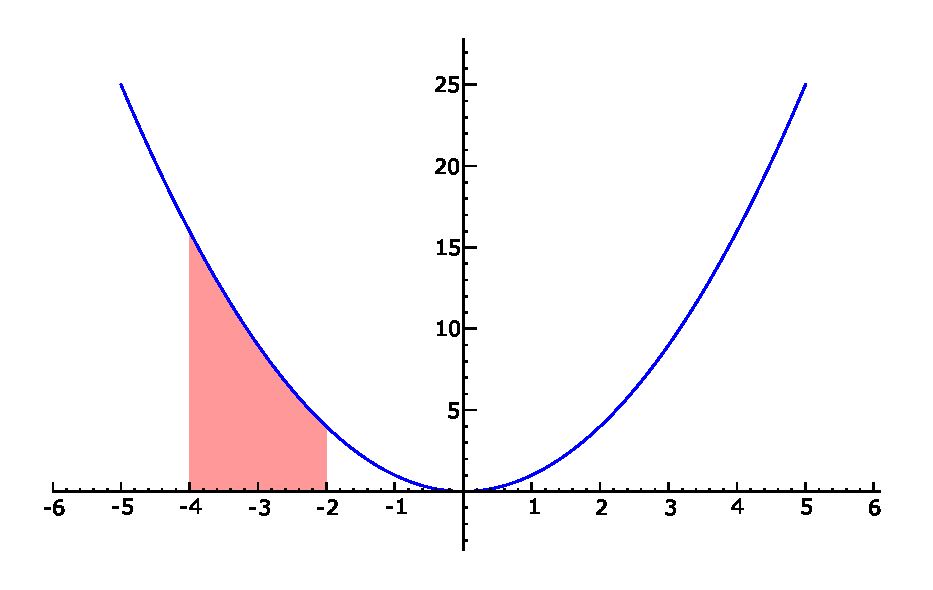
\includegraphics[width=0.45\textwidth]{img/9May2008img1.eps}
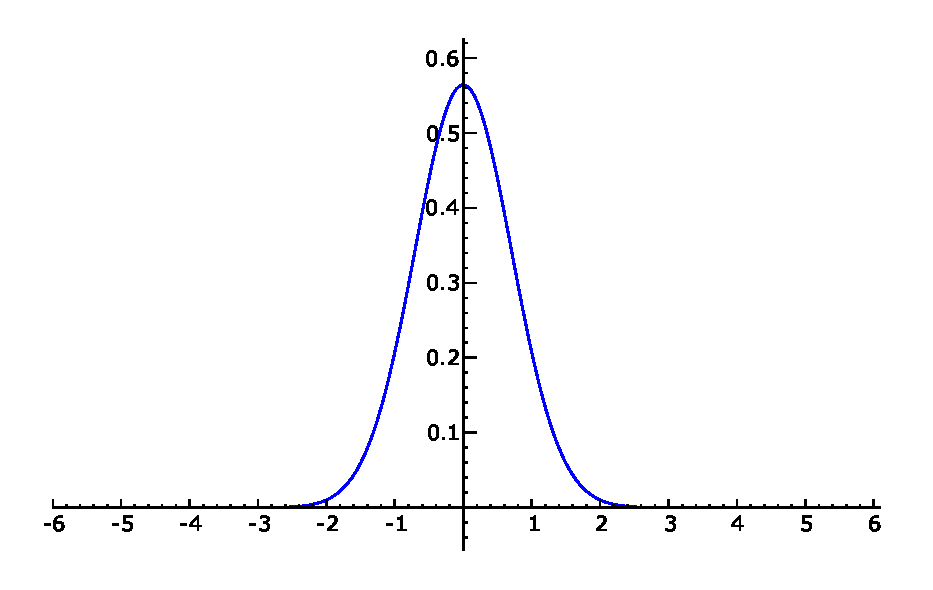
\includegraphics[width=0.45\textwidth]{img/9May2008img2.eps}
\caption{On the left, convolution with $x^2$; on the right, the Gaussian Kernel.}\label{img:9May2008:img1}\label{img:9May2008:img2}
\end{figure}

%% \begin{figure}
%% \subfigure[Convolution with $x^2$]{\label{img:9May2008:img1}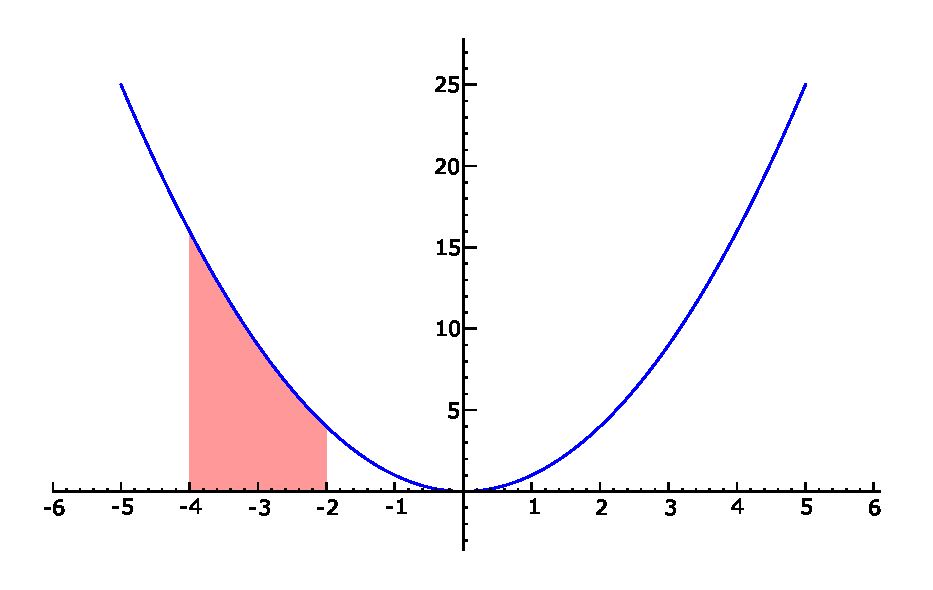
\includegraphics[width=0.45\textwidth]{img/9May2008img1.eps}}
%% \subfigure[Gaussian Kernel]{\label{img:9May2008:img2}w
%% \end{figure}

\begin{ex}
Let $g(x)=x^2$, consider the convolution
$(f*g)(x)$. Convolution is just sliding $f$ along the $x$ 
axis. You can see the integral as the red shaded region of
figure \eqref{img:9May2008:img1}.
\end{ex}

\begin{ex}
Let $f(x)=\exp(-x^2)$ and $g(x)=x^2$. Then we first
normalize $f(x)$ by introducing
$\widetilde{f}(x)=f(x)/\sqrt{\pi}$ so we see
\begin{equation}
\int\widetilde{f}(x)dx = 1.
\end{equation}
This is a special function called the Gaussian
Kernel\index{Gaussian Kernel}\marginpar{Gaussian Kernel}
\begin{equation}
  \addtolength{\fboxsep}{5pt}
   \boxed{
   \begin{gathered}
     \widetilde{f}(x) = \frac{e^{-x^2}}{\sqrt{\pi}}
   \end{gathered}
   }
\end{equation}
For $|x|\geq 4$, $\widetilde{f}(x)\leq 6.4\times
10^{-8}$. The values of $\widetilde{f}(x)$ that really
matter are between $[x-4,x+4]$. One can see this reflected
in the plot of the Gaussian in figure \eqref{img:9May2008:img2}.

Suppose we shrink this down to
$[x-\varepsilon,x+\varepsilon]$ for small $\varepsilon$ by
scaling or ``dilating'' $f$. We do this, given $\int
f(x)dx=1$, we define\marginpar{Scaling or Dilations} the 
\textbf{scaling}\index{Scaling} or \textbf{dilation}\index{Dilation}
of $f$ is given as
\begin{equation}
f_{\varepsilon}(x) = \frac{1}{\varepsilon}f\left(\frac{x}{\varepsilon}\right)
\end{equation}
For $f(x)=\exp(-x^2)/\sqrt{\pi}$, we have
\begin{equation}
f_{\varepsilon}(x) = \frac{1}{\varepsilon\sqrt{\pi}}\exp(-(x/\varepsilon)^2).
\end{equation}
As $\varepsilon$ gets smaller, the peak gets higher, so
$f_{\varepsilon}(x)\leq(6.4\times10^{-8})/\varepsilon$ for
$|x|\geq4\varepsilon$. What then is
\begin{subequations}
\begin{align}
(f_{\varepsilon}*g)(x) &= \frac{1}{\varepsilon\sqrt{\pi}}\int\exp\left[-\left(\frac{x-y}{\varepsilon}\right)^{2}\right]g(y)dy\\
&\approx \frac{1}{\varepsilon\sqrt{\pi}}\int^{x+4\varepsilon}_{x-4\varepsilon}\exp\left[-\left(\frac{x-y}{\varepsilon}\right)^{2}\right]g(y)dy
\end{align}
\end{subequations}
\end{ex}
